\documentclass[]{beamer}
% ignorenonframetext
\usetheme{Dresden}
\setbeamertemplate{caption}[numbered]
\setbeamertemplate{caption label separator}{:}
\setbeamercolor{caption name}{fg=normal text.fg}
\usepackage{amssymb,amsmath}
\usepackage{ifxetex,ifluatex}
\usepackage{lmodern}
\usepackage{metalogo}

\ifxetex
  \usepackage{fontspec,xltxtra,xunicode}
  \defaultfontfeatures{Mapping=tex-text,Scale=MatchLowercase}
  \newcommand{\euro}{€}
\else
  \ifluatex
    \usepackage{fontspec}
    \defaultfontfeatures{Mapping=tex-text,Scale=MatchLowercase}
    \newcommand{\euro}{€}
  \else
    \usepackage[T1]{fontenc}
    \usepackage[utf8]{inputenc}
      \fi
\fi
% use upquote if available, for straight quotes in verbatim environments
\IfFileExists{upquote.sty}{\usepackage{upquote}}{}
% use microtype if available
\IfFileExists{microtype.sty}{\usepackage{microtype}}{}
\usepackage{url}

% Comment these out if you don't want a slide with just the
% part/section/subsection/subsubsection title:
\AtBeginPart{
  \let\insertpartnumber\relax
  \let\partname\relax
  \frame{\partpage}
}
\AtBeginSection{
  \let\insertsectionnumber\relax
  \let\sectionname\relax
  \frame{\sectionpage}
}
\AtBeginSubsection{
  \let\insertsubsectionnumber\relax
  \let\subsectionname\relax
  \frame{\subsectionpage}
}

\setlength{\parindent}{0pt}
\setlength{\parskip}{6pt plus 2pt minus 1pt}
\setlength{\emergencystretch}{3em}  % prevent overfull lines
\setcounter{secnumdepth}{0}

\title{\LaTeX \ für Einsteiger}
\author{Valentin Heinz}
\date{\today}

\begin{document}

\maketitle
\title{Einführung}
\begin{frame}{Vorstellung}

\begin{itemize}
\itemsep1pt\parskip0pt\parsep0pt
\item
  herzlich willkommen! :)
\item
  Valentin Heinz
  (\href{mailto:Valentin.Heinz@hhu.de}{\nolinkurl{Valentin.Heinz@hhu.de}})
\item
  Computerlinguistik im Master (Abschlussarbeit fehlt noch)
\item
  ich mag \LaTeX \ und Gestaltung
\item
  ich unterrichte und programmiere gerne
\end{itemize}

\end{frame}

\begin{frame}{Praktisches, Fragen}

\begin{itemize}
\itemsep1pt\parskip0pt\parsep0pt
\item
  Sie oder Du?
\item
  haben Sie einen Laptop dabei? Haben Sie Strom?
\item
  wann machen wir Mittagspause?
\end{itemize}

\end{frame}

\begin{frame}{Überblick}

\begin{itemize}
\itemsep1pt\parskip0pt\parsep0pt
\item
  der heutige Inhalt besteht aus folgenden Teilen:

  \begin{itemize}
  \itemsep1pt\parskip0pt\parsep0pt
  \item \LaTeX-Geschichte
  \item \LaTeX-Funktionsweise
  \item \LaTeX-Dokumentstruktur
  \item mehr Befehle
  \item Schriftformatierung
  \item mehr Struktur
  \item Übungen
  \end{itemize}
\item
  wie sieht die Struktur eines Teils aus?

  \begin{itemize}
  \itemsep1pt\parskip0pt\parsep0pt
  \item
    Einstieg: Wiederholung, Fragen
  \item
    Inhalte werden idealer Weise durch den Theorieteil, Praxisteil und Übungen vermittelt
  \end{itemize}
\end{itemize}

\end{frame}

\begin{frame}{Motivation}

\begin{itemize}
\itemsep1pt\parskip0pt\parsep0pt
\item
  oder: warum gebe ich diesen Kurs?
\item
  es gibt viele Übersichten, Bücher, Webseiten usw. zu \LaTeX, aber kaum
  praktische Kurse
\item
  in Seminaren sind die Lernerfolge gut überprüfbar
\item
  die Hilfestellung ist direkt und passend
\item
  Erfahrungsaustausch, Tipps \& Tricks bündeln
\end{itemize}

\end{frame}

\begin{frame}{Vorstellung 2}

\begin{itemize}
\itemsep1pt\parskip0pt\parsep0pt
\item
  Fachsemester
\item
  Vorstellungsrunde:

  \begin{itemize}
  \itemsep1pt\parskip0pt\parsep0pt
  \item
    wie heißen Sie?
  \item
    ihre nächste große Arbeit ist \ldots{} ?
  \item
    welche fachliche Ausrichtung haben Sie?
  \item
    welche Schwerpunkte haben Sie?
  \end{itemize}
\end{itemize}

\end{frame}

\begin{frame}{Dokumenttypen}

\begin{itemize}
\itemsep1pt\parskip0pt\parsep0pt
\item
  Bedarfsevaluation
\item
  welche Dokumenttypen sind für Sie relevant?

  \begin{itemize}
  \itemsep1pt\parskip0pt\parsep0pt
  \item
    Buch
  \item
    Artikel/Hausarbeit
  \item
    Präsentation
  \item
    Magazin
  \item
    Konferenzposter
  \item
    Bewerbungsunterlagen
  \item
    Lebenslauf
  \item
    Umfragebogen
  \item
    Brief
  \item
    Gedicht, Notensatz, Theaterstück, \ldots{}
  \end{itemize}
\end{itemize}

\end{frame}

\begin{frame}{Ziele}

\begin{itemize}
\itemsep1pt\parskip0pt\parsep0pt
\item
  \LaTeX \ lernen und dann \textbf{üben}
\item
  einfacheres, schöneres und effizienteres wissenschaftliches Arbeiten
  mit \LaTeX
\item
  Probleme mit \LaTeX \ selber lösen
\item
  einen Überblick über die Möglichkeiten und das Ökosystem bieten
\item
  Fragen richtig stellen, Hilfe zur Selbsthilfe
\end{itemize}

\end{frame}

\begin{frame}{Eigenleistung}

\begin{itemize}
\itemsep1pt\parskip0pt\parsep0pt
\item
  selbsterstelltes Cheatsheet
\item
  eigenständig erstellte Arbeit, diese beinhaltet:

  \begin{itemize}
  \itemsep1pt\parskip0pt\parsep0pt
  \item
    eine aussagenlogische Formel
  \item
    eine Tabelle mit einer Kopfzeile und mindestens drei normalen Zeilen
  \item
    etwas Fließtext
  \item
    ein Zitat mit Quellenangabe
  \item
    eine besonderheit deines Spezialgebiets (z.B. phonetische
    Transkiption)
  \item
    das Literaturverzeichnis
  \item
    wichtig: Kommentare, welcher Teil des Quelltextes dem jeweiligen
    obigen Teil entspricht
  \end{itemize}
\item
  \scriptsize keine Panik, folgendes sieht nach mehr aus, als es ist! Dennoch stelle
  ich damit sicher, dass Sie mit \LaTeX \ arbeiten können.\normalsize
\end{itemize}

\end{frame}


\title{Geschichte}
\begin{frame}{\LaTeX-Geschichte}
\begin{figure}[htbp]
\centering
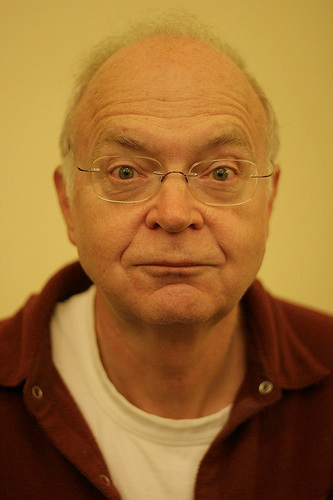
\includegraphics[width=\textwidth*0.8,height=\textheight*0.8,keepaspectratio]{../../img/knuth.jpg}
\caption{Donald E. Knuth}
\end{figure}

\end{frame}

\begin{frame}{Donald E. Knuth}

\begin{itemize}
\itemsep1pt\parskip0pt\parsep0pt
\item
  emeritierter Professor (Stanford)
\item
  fast jährliche Preise und Auszeichnungen seit 1970 bis heute
\item
  25 Ehrendoktortitel
\item
  Knuth-Preis: außergewöhnliche Leistungen in den Grundlagen der
  Informatik
\item
  Asteroid: (21656) Knuth
\end{itemize}

\end{frame}

\begin{frame}{Trivia?}

\begin{itemize}
\itemsep1pt\parskip0pt\parsep0pt
\item
  ab 1. Januar 1990: mehr Konzentration auf Arbeit, nutzt keine E-Mails
  mehr
\item
  Korrektheit ist sehr wichtig: verschickt Schecks über 2.56\$ für
  gefundene Fehler
\item
  (wg. der Angst vor Scheckbetrug benutzt er nun die digitale Währung
  einer fiktiven Bank, zahlt das Guthaben aber auch gerne aus)
\end{itemize}

\end{frame}

\begin{frame}{verstehen Sie Spaß?}

\begin{figure}[htbp]
\centering
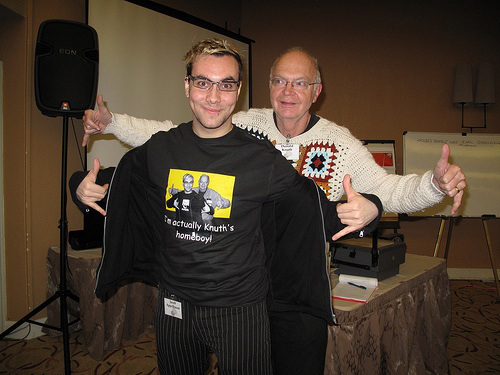
\includegraphics[width=\textwidth*0.8,height=\textheight*0.8,keepaspectratio]{../../img/knuth-applebaum.jpg}
\caption{mit Jacob Applebaum}
\end{figure}

\end{frame}

\begin{frame}{Ein Buch über Comiler}

\begin{itemize}
\itemsep1pt\parskip0pt\parsep0pt
\item
    Knuth (noch Student im Hauptstudium) schreibt ein Buch über Compiler
\item
    \textit{Do you mind if I make this book a little bit longer, because I think there's a need for explaining these things in somewhat more detail.}
\item
    \textit{They said, ‚Oh no, go right ahead. Make it as long as you feel necessary.'}
\item
  Ergebnis: 3900 Seiten (1968)
\end{itemize}

\end{frame}

\begin{frame}{The Art of Computer Programming}

\begin{itemize}
\itemsep1pt\parskip0pt\parsep0pt
\item
  Band 1: 1968, Band 5 (von 7): 2020
\item
  legendäres Grundlagenwerk
\item
  eigener theoretischer, idealer Computer MIX, eigene Assemblersprache
  MIXAL
\item
  Themen: Algorithmen und Datenstrukturen (und Zahlentheorie, Suchen,
  Sortieren, uvm.)
\end{itemize}

\end{frame}

\begin{frame}{\TeX \ entsteht}

\begin{itemize}
\itemsep1pt\parskip0pt\parsep0pt
\item
  Überarbeitung von Band 2: Knuth erfindet \TeX
\item
  Schriftartendesign, Satztechnik, \ldots{}
\item
  Bücher über \TeX \ in \TeX: Spezifikation und Benutzung
\item
  Erklärung von Verfahren, z.B.: Worttrennungsalgorithmus
\end{itemize}

\end{frame}

\begin{frame}{\LaTeX \ und \LaTeXe}

\begin{itemize}
\itemsep1pt\parskip0pt\parsep0pt
\item
  1980: Leslie \emph{La}mport entwickelt Makros für \TeX: \emph{La}TeX
\item
  1990: Lamport beendet die Entwicklung. \LaTeX \ wird fortgeführt.
\item
  1994: \LaTeXe ist die Fortführung von \LaTeX
\item
  bedeutet: \LaTeX \ ist älter als Unicode
\end{itemize}

\end{frame}

\begin{frame}{Exkurs: Unicode}

\begin{itemize}
\itemsep1pt\parskip0pt\parsep0pt
\item
  internationaler Standard zur Zeichenkodierung (Version 1.0.0: Oktober
  1991)
\item
  soll \emph{jedes} sinntragende Zeichen umfassen
\item
  alle bekannten Schriftkulturen und Zeichensysteme
\item
  ein Beispiel für einen Codepunkt: \texttt{U+1F600} (welcher ist das?)
\item
  UTF-8: 8-bit Kodierung für Unicode-Zeichen, sehr verbreitet
\item
  Internet Engineering Task Force: neue Protokolle müssen UTF-8 können
\end{itemize}

\end{frame}

\begin{frame}{Aufgaben}

\begin{itemize}
\itemsep1pt\parskip0pt\parsep0pt
\item
  mit dem Hintergrund von \LaTeX \ und Unicode-Wissen, versuchen Sie
  folgendes herauszufinden:
\item
  was ist pdfTeX?
\item
  was ist \XeTeX? Inwiefern ist \XeTeX \ besser als \LaTeX?
\item
  was ist \LuaTeX? Was macht \LuaTeX \ anders als pdfTeX?
\end{itemize}

\end{frame}


\title{Pause}
\begin{frame}{Pause}

\Huge Pause?

\end{frame}


\title{Methodik}
\begin{frame}{WYSIWYG}

\begin{itemize}
\itemsep1pt\parskip0pt\parsep0pt
\item
  What You See Is What You Get

  \begin{itemize}
  \itemsep1pt\parskip0pt\parsep0pt
  \item
    Beispiele: Word/OpenOffice/Libreoffice
  \item
    Benutzer: Inhalt eingeben → Formatierung
  \item
    Programm: nach Umgebung → Layouting der Eingabe
  \item
    Prozess: nach und nach
  \end{itemize}
\item
  man legt fest, wie eine Überschrift \emph{aussieht}
\item
  man legt \emph{nicht} fest, was (strukturell!) eine Überschrift
  \emph{ist}
\item
  (aber: Formatvorlagen)
\end{itemize}

\end{frame}

\begin{frame}{WYSIWYM}

\begin{itemize}
\itemsep1pt\parskip0pt\parsep0pt
\item
  What You Get Is What You Mean
\item
  Auszeichnungssprachen: \emph{logische} Auszeichnung von
  \emph{Strukturen}
\item
  Beispiel: HTML

  \begin{itemize}
  \itemsep1pt\parskip0pt\parsep0pt
  \item
    Titel:
    \texttt{\textless{}title\textgreater{}Ich\ bin\ der\ Titel\textless{}/title\textgreater{}}
  \item
    kursiv:
    \texttt{\textless{}i\textgreater{}ich\ bin\ kursiv\textless{}/i\textgreater{}}
  \end{itemize}
\item
  Beispiel: \LaTeX
  \begin{itemize}
  \itemsep1pt\parskip0pt\parsep0pt
   \item 
    Titel:
    \texttt{\textbackslash{}title\{Ich\ bin\ auch\ ein\ Titel\}}
  \item
    kursiv:
    \texttt{\textbackslash{}textit\{und\ ich\ bin\ auch\ kursiv\}}
  \end{itemize}
\end{itemize}

\end{frame}

\begin{frame}{\LaTeX-Textsatz}

\begin{itemize}
\itemsep1pt\parskip0pt\parsep0pt
\item
  man legt fest, was vom Text z.B. eine Überschrift ist
\item
  man legt aber \emph{nicht} fest, wie eine Überschrift aussieht
\item
  Berufe: Typograph, Schriftsetzer, Designer
\item
  Vorgang: erst schreiben (Quelltext) und auszeichnen, dann layouten
  \emph{lassen}
\item
  \texttt{kompilieren}: Übersetzung vom Quelltext zum fertigen Dokument
\end{itemize}

\end{frame}

\begin{frame}{gefühlte Vorteile}

\begin{itemize}
\itemsep1pt\parskip0pt\parsep0pt
\item
  hochwertige Typographie (was bedeutet das??)
\item
  Dokumente sind leicht unterteilbar in einzelne Dateien
\item
  einfache Arbeit mit Referenzen und Zitierstilen
\item
  Sachen die in Word nicht funktioniert haben

  \begin{itemize}
  \itemsep1pt\parskip0pt\parsep0pt
  \item
    Bsp.: Pragmatikhandout: mehrfache Potenz. \LaTeX:
    \texttt{\textbackslash{}(\ a\^{}\{b\^{}\{c\^{}\{d\}\}\}\ \textbackslash{})}
  \end{itemize}
\item
  einfaches Aufschreiben von beliebig komplexen mathematischen Formeln
\item
  Text (besonders UTF-8) ist toll, weil universell und immer zugänglich
\end{itemize}

\end{frame}

\begin{frame}{Einarbeitungszeit}

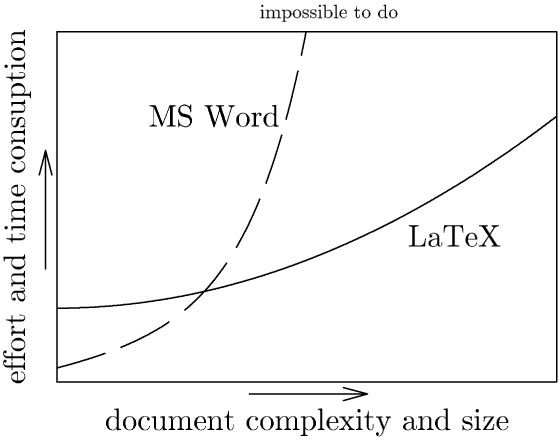
\includegraphics[width=\textwidth*0.8,height=\textheight*0.8,keepaspectratio]{../../img/miktex.png} Quelle:
\url{http://www.pinteric.com/miktex.html}

\end{frame}

\begin{frame}{Vorteile, die man später bemerkt}

\begin{itemize}
\itemsep1pt\parskip0pt\parsep0pt
\item
  Skalierbarkeit: „Bücher schreibt man in \LaTeX!``
\item
  kostenlos und bleibt es
\item
  Freiheit: keine Hersteller- bzw. Lizenzbindung (MS-Office-Preise,
  SPSS-Preise)
\item
  Akzeptanz \& Verbreitung

  \begin{itemize}
  \itemsep1pt\parskip0pt\parsep0pt
  \item
    kollaboratives Arbeiten ist leichter (jeder kann seinen Teil
    unabhängig einbinden)
  \item
    (Abschluss)arbeiten in der Mathematik, Naturwissenschaft und Technik
  \item
    Paper: \LaTeX-Templates von Journals
  \end{itemize}
\end{itemize}

\end{frame}

\begin{frame}{Nachteile}

\begin{itemize}
\itemsep1pt\parskip0pt\parsep0pt
\item
  schwieriger Einstieg
\item
  steilere Lernkurve
\item
  \ldots{} dafür gibt es dieses Seminar! Schildert mir Nachteile, die
  mir nicht einfallen)
\item
  Schriftarten (dafür gibt es aber \XeTeX \ und \LuaTeX \ usw.)
\end{itemize}

\end{frame}


\title{Pause}
\begin{frame}{Pause}

\Huge Pause?

\end{frame}


\title{Struktur}
\begin{frame}{\LaTeX-Praxis}

\end{frame}

\begin{frame}{Editor}

Um erste \LaTeX-Erfahrungen zu machen

\begin{itemize}
\itemsep1pt\parskip0pt\parsep0pt
\item
  rufen Sie \url{https://www.overleaf.com/} auf
\item
  dort schalten Sie links oben auf \texttt{Source}
\item
  dann schalten Sie rechts oben den \texttt{Preview}-Schalter auf
  \texttt{Manual}
\item
  dann löschen Sie das Dokument
\end{itemize}

\end{frame}

\begin{frame}{erste (!) Dokumenttypen}

Sie müssen bei jedem \LaTeX-Dokument den Dokumenttypen angeben:
\begin{itemize}
\item \texttt{article} Journals, usw.
\item \texttt{report} längere Berichte, kurze Bücher, Diplomarbeiten
\item \texttt{book} richtige Bücher
\item \texttt{letter} Briefe
\item \texttt{beamer} Präsentationen (siehe \LaTeX/Präsentationen)
\end{itemize}

Weiterhin müssen Sie definieren, wo unser Dokument anfängt.

\end{frame}

\begin{frame}[fragile]{Minimalbeispiel (Struktur)}

\begin{verbatim}

\documentclass{article}

\begin{document}
    Hello World!
\end{document}
\end{verbatim}

\begin{itemize}
\item Dokumentaufbau (Nicht-Dokument, Dokument, Text)
\item Frage: was ist was?
\end{itemize}
\end{frame}

\begin{frame}[fragile]{Syntax}

\begin{itemize}
\itemsep1pt\parskip0pt\parsep0pt
\item
    Ab und an werde ich die Befehlssyntax näher besprechen, wie in diesen
    Beispielen
\end{itemize}

\begin{verbatim}
\befehl{PARAMETER}

\begin{PARAMETER}
\end{PARAMETER}
\end{verbatim}

\end{frame}

\begin{frame}[fragile]{Keine Probleme?}

\begin{itemize}
\itemsep1pt\parskip0pt\parsep0pt
\item
  Finden Sie Probleme in diesem Beispiel?
\end{itemize}

\begin{verbatim}
\documentclass{article}
\begin{document}
Außerdem und überhaupt: „wir“ wollen mehr!
\end{document}
\end{verbatim}

\end{frame}

\begin{frame}{Probleme: Umlaute und Sonderzeichen}

\begin{itemize}
\itemsep1pt\parskip0pt\parsep0pt
\item
  Anführungszeichen
\item
  für deutschsprachige Arbeiten unübliche Ränder und Abstände
\item
  keine Kommentare
\end{itemize}

\end{frame}


\title{verbesserte Struktur}

\begin{frame}{Dokumenttypen des Koma-Script-Pakets (Markus Kohm)}

\begin{itemize}
\itemsep1pt\parskip0pt\parsep0pt
\item
  \texttt{scrartcl} Journals, usw.
\item
  \texttt{scrreprt} längere Berichte, kurze Bücher, Diplomarbeiten
\item
  \texttt{scrbook} richtige Bücher
\item
  \texttt{scrlttr2} Briefe
\item
  \texttt{beamer} wer weiß das noch?
\end{itemize}

\end{frame}

\begin{frame}{Ein besseres Beispiel}

\begin{itemize}
\itemsep1pt\parskip0pt\parsep0pt
\item besuchen Sie die Seminarseite:
\item
  \url{https://github.com/inktrap/LaTeXKurs}
\item
  laden Sie: \texttt{01-hello-world.tex} herunter.
\item
  kopieren Sie den Inhalt in \texttt{overleaf}
\end{itemize}

\end{frame}

\begin{frame}{Bestandteile}

\begin{itemize}
\itemsep1pt\parskip0pt\parsep0pt
\item
  Kommentare
\item
  Encoding definieren: UTF-8 (ISO 8859-1)
\item
  Spracheinstellung: babel
\item
  Pakete einbinden. Syntax:
  \texttt{\textbackslash{}usepackage{[}OPTIONEN{]}\{PAKETNAME\}}
\item
  Paketinformationen: \url{https://www.ctan.org/}
\end{itemize}

\end{frame}

\begin{frame}{Änderungen}

\begin{itemize}
\itemsep1pt\parskip0pt\parsep0pt
\item
  was passiert, wenn Sie einen anderen Dokumenttypen wählen?
\item
  ihre Erwartung: wie würden Sie einen Absatz einfügen? Was passiert?
\item
  binden Sie das Packet \texttt{ellipsis} ein und finden Sie heraus, was
  es macht \ldots{}
\item
  wie kann man die neue Rechtschreibung und Din-A4 verwenden? Hinweis:
  Dokumenttyp
\end{itemize}
\end{frame}

\begin{frame}{Übungen}

\begin{itemize}
\itemsep1pt\parskip0pt\parsep0pt
\item
  Methode: Pairprogramming
\item
  eine Person programmiert (Driver), die andere schaut zu und denkt mit
  (Navigator)
\item
  der Navigator denkt auch eigenständig über das Problem nach
\item
  versteht der Navigator einen Schritt des Drivers nicht, kann er direkt
  nachfragen
\item
  steht der Driver vor einem Problem, kann er dieses dem Navigator
  beschreiben
\end{itemize}

\end{frame}

\begin{frame}{Paarprogrammierung 1: Durcheinander}

\begin{itemize}
\itemsep1pt\parskip0pt\parsep0pt
\item
  laden Sie
  \url{01-hello-world_wrong-order.tex}
\item
  erstens: Durcheinander sortieren, dann
\item
  zweitens: damit das nicht wieder passiert, erweitern Sie das Template
  um Kommentare
\end{itemize}

\end{frame}

\begin{frame}{Paarprogrammierung 2: Fehler}

\begin{itemize}
\itemsep1pt\parskip0pt\parsep0pt
\item
  tauschen Sie die Rollen
\item
  laden Sie
  \url{01-hello-world_wrong-cmd.tex}
  herunter
\item
  erklären Sie im Gespräch/zusammen mit Ihrem Nachbarn die
  Fehlermeldung(en)
\item
  korrigieren Sie alle syntaktischen Fehler
\end{itemize}

\end{frame}


\title{Pause}
\begin{frame}{Pause}

\Huge Pause?

\end{frame}


\title{Syntax}
\begin{frame}{Zusammenfassung der Syntax}

\end{frame}

\begin{frame}{Syntax}

\begin{itemize}
\itemsep1pt\parskip0pt\parsep0pt
\item
  \texttt{PARAMETER} sind Argumente
\item
  \texttt{PARAMETER} sind nicht immer \texttt{OPTIONEN}
\item
  \texttt{OPTIONEN} sind optionale \texttt{PARAMETER}
\item
  unser erster Befehl: \texttt{\textbackslash{}documentclass\{\}}.
  Syntax:
  \texttt{\textbackslash{}documentclass{[}OPTIONEN{]}\{PARAMETER\}}
\item
  unsere erste Umgebung: durch \texttt{\textbackslash{}begin\{\}} und
  \texttt{\textbackslash{}end\{\}}. Syntax:
\end{itemize}

\end{frame}

\begin{frame}[fragile]{Befehlsarten}

\begin{verbatim}
% nicht optional
\befehl{PARAMETER}

% optional
\befehl[OPTIONEN]

% beides
\befehl[OPTIONEN]{PARAMETER}
\end{verbatim}

\end{frame}

\title{Schrift}
\begin{frame}[fragile]{Textformatierung}

\begin{itemize}
\itemsep1pt\parskip0pt\parsep0pt
\item
  Die Textformatierung findet mit einem Schalter statt.
\item
  Dieser nimmt keine Parameter und bleibt bei Größenangaben aktiv, bis
  ein anderer Schalter aktiv wird.
\item
  Hinweis: \texttt{\textbackslash{}LaTeX}, etc. ist kein Schalter,
  sondern nur ein Textbefehl
\end{itemize}

Syntax:

\begin{verbatim}
% schalter ist nicht aktiv
\schaltername
% schalter ist aktiv
\end{verbatim}

\end{frame}

\begin{frame}{Größe}

\begin{itemize}
\itemsep1pt\parskip0pt\parsep0pt
\item
  \texttt{\textbackslash{}tiny}
\item
  \texttt{\textbackslash{}scriptsize}
\item
  \texttt{\textbackslash{}footnotesize}
\item
  \texttt{\textbackslash{}small}
\item
  \texttt{\textbackslash{}normalsize}
\item
  \texttt{\textbackslash{}large}
\item
  \texttt{\textbackslash{}Large}
\item
  \texttt{\textbackslash{}LARGE}
\item
  \texttt{\textbackslash{}huge}
\item
  \texttt{\textbackslash{}Huge}
\end{itemize}

\end{frame}

\begin{frame}{Übung}

\begin{itemize}
\itemsep1pt\parskip0pt\parsep0pt
\item
  betrachten Sie folgende Geschichte:
\item
  \texttt{tiny\ and\ huge\ are\ walking\ to\ the\ small\ house\ of\ footnotesize.\ tiny\ says:\ “this\ is\ too\ Huge\ for\ me”\ and\ huge\ thinks\ thats\ not\ normalsize\ either}
\item
  formatieren Sie das Wort der ersten Größe mit der letzten vorkommenden
  Größe.
\item
  d.h.: tiny mit normalsize, huge mit huge, usw.
\end{itemize}

\end{frame}

\begin{frame}{Größe als Umgebung}

\begin{itemize}
\itemsep1pt\parskip0pt\parsep0pt
\item
  die Größe kann auch per Umgebung definiert werden:
  \texttt{\textbackslash{}begin\{scriptsize\}\ Ein\ kleiner\ Satz.\ \textbackslash{}end\{scriptsize\}\ Ich\ bin\ wieder\ normal.}
\item
  dies ist häufig viel leichter zu überschauen, da man die Umgebung
  bewusst beendet.
\end{itemize}

\end{frame}

\begin{frame}[fragile]{Schriftformatierung und Übung}

Übernehmen Sie folgende Formatierungsangaben in Ihr Cheatsheet:

\begin{verbatim}
Laut
\textsc{Gaius Iulius Caesar} sollte man neue Begriffe
\textit{kursiv} schreiben und nicht
\textbf{fett}, besonders
\texttt{Schreibmaschinen} sind eher
\texttt{\textbf{\textit{total}}} unnötig.
\end{verbatim}

\end{frame}

\begin{frame}{Hausaufgabe: Farben}

\begin{itemize}
\itemsep1pt\parskip0pt\parsep0pt
\item
  finden Sie heraus, wie sie Text farbig gestalten können
\item
  zeigen Sie dies morgen an einem Beispiel
\end{itemize}

\end{frame}


\title{Pause}
\begin{frame}{Pause}

\Huge Pause?

\end{frame}


\title{mehr Struktur}
\begin{frame}[fragile]{Kapitel}

\begin{verbatim}
% 1
\section[ALTERNATIV]{ABSCHNITT}

% 2
\section*{ABSCHNITT}
\end{verbatim}

\begin{itemize}
\itemsep1pt\parskip0pt\parsep0pt
\item
  tragen Sie etwas für \texttt{ABSCHNITT} ein.
\item
  \texttt{ALTERNATIV} ist die Kurzform, die auch z.B. im
  Inhaltsverzeichnis auftaucht
\item
  wir haben bereits gesehen, dass eine \texttt{{[}OPTION{]}} auch
  weggelassen werden kann.
\item
  was bewirkt das \texttt{*} Sternchen in \texttt{2}?
\end{itemize}

\end{frame}

\begin{frame}[fragile]{Unterkapitel}

\begin{itemize}
\itemsep1pt\parskip0pt\parsep0pt
\item
  wir wollen nun Abschnitte und Unterabschnitte
\end{itemize}

\begin{verbatim}

% 3
\section[ALTERNATIV]{ABSCHNITT}

% 4
\subsection[ALTERNATIV]{UNTERABSCHNITT}
\end{verbatim}

\end{frame}

\begin{frame}{Übungen}

\begin{itemize}
\itemsep1pt\parskip0pt\parsep0pt
\item
  wie würden sie den Unterabschnitt von einem Unterabschnitt bilden?
\item
  wie lange funktioniert das? Was passiert dann?
\end{itemize}

\end{frame}

\begin{frame}[fragile]{Nummerierte Listen}

\begin{verbatim}
% 5
\begin{enumerate}
    \item ITEM 1
    \item ITEM 2
    \item ITEM 3
\end{enumerate}
\end{verbatim}

\end{frame}

\begin{frame}[fragile]{Nicht nummerierte Listen}

\begin{verbatim}
% 6
\begin{itemize}
    \item ITEM 1
    \item ITEM 2
    \item ITEM 3
\end{itemize}
\end{verbatim}

\end{frame}

\begin{frame}{Übungen}

\begin{itemize}
\itemsep1pt\parskip0pt\parsep0pt
\item
  was passiert, wenn Sie ein \texttt{\textbackslash{}end\{enumerate\}}
  oder \texttt{\textbackslash{}end\{itemize\}} vergessen?
\item
  was passiert, wenn Sie ein \texttt{\textbackslash{}begin\{enumerate\}}
  oder \texttt{\textbackslash{}begin\{itemize\}} vergessen?
\item
  kann ein \texttt{\textbackslash{}item} auch alleine stehen? Also:
  nicht in einer Liste?
\item
  was ist, wenn eine Liste kein \texttt{\textbackslash{}item} hat?
\item
  was passiert, wenn Sie nummerierte Listen schachteln? Wenn das geht,
  wie weit geht das?
\item
  was passiert, wenn Sie nicht-nummerierte Listen schachteln? Wenn das
  geht, wie weit geht das?
\item
  erinnern Sie sich an
  \texttt{\textbackslash{}section*\{Nicht-nummerierte\ Überschrift\}}?
  Geht dies auch bei nummerierten Listen?
\end{itemize}

\end{frame}

\begin{frame}[fragile]{Blockzitate}
\begin{itemize}
\itemsep1pt\parskip0pt\parsep0pt
\item
  Blockzitate sind auch nur Umgebungen, genau wie \texttt{document},
  \texttt{enumerate}, \texttt{itemize}, \ldots{}
\end{itemize}
\begin{verbatim}

\begin{quote}
Ich bin ein Blockzitat
\end{quote}
\end{verbatim}
\end{frame}

\begin{frame}[fragile]{Ende des ersten Tages}
\begin{itemize}
\itemsep1pt\parskip0pt\parsep0pt
\item vielen Dank für Ihre Aufmerksamkeit!
\item haben Sie Fragen?
\item wir üben nun noch!
\end{itemize}

\end{frame}


\end{document}
